% -*- fill-column: 52 -*-
% (local-set-key (kbd "C-c C-f") 'display-fill-column-indicator-mode)
\chapter{Operátorok}
Van még szintaktikus cukor bizonyos struktúrákon:
ezek az \emph{operátorok}. Amikor például leírunk
egy olyan matematikai kifejezést, hogy $2a+bc$, vagy
a szorzásokat csillaggal (\pr{*}) jelölve,
\pr{2*a+b*c}, akkor a szorzás és összeadás műveletek
az argumentumaik \emph{között} szerepelnek. Ezeket
hívjuk \emph{infix} (,,közbülső'') operátoroknak. Ha
egy ilyen kifejezést a szokásos \emph{prefix}
(,,elülső'') funktorokkal szeretnénk leírni, akkor
ezt kapnánk:
\index{operátor}
\index{operátor!prefix}
\index{operátor!infix}
\begin{query}
+(*(2, a), *(b, c))
\end{query}
Vannak nyelvek, amelyek ezt preferálják, és vannak
olyanok, amelyek a \emph{posztfix} (,,hátulsó'')
operátorokat:
\index{operátor!posztfix}
\begin{query}
((2, a)*, (b, c)*)+
\end{query}
... de a Prolog ezekre a megszokott infix
jelöléseket támogatja.

\begin{infobox*}{}{pre-, in- és posztfix}
Kizárólag prefix operátorokkal működnek a
\emph{Lisp} nyelvcsalád nyelvei (Common Lisp,
Scheme, Clojure, Racket etc.) Ezeknél a funktor neve
is a zárójelen belülre kerül, tehát a fenti példából
ez lesz: {\tt (+ (* 2 a) (* b c))}
\index{Lisp}

Ennek az egyik előnye a következetesség, a másik
pedig, hogy a műveletek kiterjeszthetőek több
argumentumra. Lispben például értelmes a {\tt (+ 1 2
  3 4 5)} kifejezés, amelynek értéke 15.

Kizárólag posztfix operátorokkal működnek a
\emph{veremnyelvek}, mint pl.~a Forth vagy a
PostScript. Itt minden operátornak csak egyféle
aritása lehet, de cserébe megszabadulunk a
zárójelektől. A fenti példa Forthban: {\tt 2 a * b c
  * +} \index{Forth}\index{veremnyelv}

Ezt hívják \emph{Reverse Polish Notation}-nek (RPN,
,,fordított lengyel jelölés''). Sok számológép is
használja; elsőre elég furcsa, de nagyon kényelmes és gyors,
ha megszokjuk.
\index{RPN}
\end{infobox*}

Tetszőleges funktorból lehet operátort csinálni. Az
egyargumentumú funktorok lehetnek pre- vagy
posztfixek, a kétargumentumúak pedig csak
infixek. Ahhoz, hogy egy ilyen kifejezést értelmezni
lehessen, még azt is kell tudni, hogy melyik operátornak
van elsőbbsége -- például a szorzást előbb kell
elvégezni, mint az összeadást, tehát elsőbbsége van.
\index{elsőbbség}

A Prologban az ilyen jellegű ,,beállításokat'' olyan
szabályokkal lehet megadni, amelyeknek nincsen feje,
csak törzse. Néhány példa operátorok definíciójára
(ezek részei az alapbeállításnak):
\begin{program}
:- op(200, fy, -).
:- op(400, yfx, *).
:- op(500, yfx, +).
:- op(1000, xfy, ',').
:- op(1200, xfx, :-).
\end{program}
Itt az első, 1 és 1200 közti szám adja meg a
\emph{precedenciá}\/t (minél kisebb, annál korábban
kell elvégezni az adott műveletet), a második a
típusát, és a harmadik magát az operátort.
\index{precedencia}

Hétféle típus létezik:
\begin{itemize}
\item \pr{xfx}, \pr{xfy}, \pr{yfx}: infix operátorok
\item \pr{fx}, \pr{fy}: prefix operátorok
\item \pr{xf}, \pr{yf}: posztfix operátorok
\end{itemize}

Ezeket úgy kell értelmezni, hogy az \pr{f} mutatja
az operátor helyét, az \pr{x} és \pr{y} pedig az
argumentumo(ka)t. Ha egy argumentum \pr{x}-el van
jelölve, akkor -- amennyiben az is egy operátoros
kifejezés -- az \pr{x} operátorának szigorúan kisebb
precedenciájúnak kell lennie az \pr{f}-nél. Ezzel
szemben az \pr{y} esetében ez nem csak kisebb lehet,
hanem egyenlő is. A zárójelezés minden előtt
elsőbbséget élvez (0 a precedenciája).

Nézzünk ez alapján egy pár példát arra, hogy a
Prolog különböző kifejezéseket hogyan elemez:
\begin{enumerate}
\item Mivel a \pr{+} operátor \pr{yfx} típusú, ha
  egy \pr{a + b + c} kifejezésem van, akkor ezt nem
  értelmezhetem úgy, hogy \pr{+(a, +(b, c))}, mert
  akkor a külső \pr{+} második argumentumában levő
  \pr{+(b, c)} kifejezés precedenciája megegyezik a
  \pr{+}-éval (hiszen az is \pr{+}). Viszont ha
  \pr{+(+(a, b), c)} módon értelmezem, ez a probléma
  nem lép fel: az első argumentumban levő \pr{+(a,
    b)} kifejezés precedenciája ugyan ugyanaz, de ez
  megengedett, mert a baloldali egy
  \pr{y}-argumentum. Tehát az \pr{yfx} operátorokat
  {\bf balról jobbra} kell zárójelezni.
\item A \pr{-a * (b + c * d)} kiértékelését először
  a zárójeles rész-szel kell kezdeni. Ezt nem
  értelmezhetem úgy, hogy \pr{*(+(b, c), d)}, mivel
  a \pr{+} precedenciája nagyobb a \pr{*}-énál, az
  \pr{yfx} szerint pedig kisebbnek vagy egyenlőnek
  kéne lennie. Ezért a helyes értelmezés a \pr{+(b,
    *(c, d))}. Ezután jön a 200-as precedenciájú
  1-argumentumú \pr{-} operátor, és végül a 400-as
  precedenciájú \pr{*}. A teljes kifejezés tehát így
  néz ki: \pr{*(-(a),+(b,*(c,d)))}.
\item A \pr{P :- Q, R, S} kifejezés helyes
  zárójelezése \pr{:-(P, ','(Q, ','(R, S)))}, mivel
  az \pr{xfy} típusú vessző operátort {\bf jobbról
  balra} kell zárójelezni, és a \pr{:-} operátor
  precedenciája a legmagasabb.
\item Mivel a \pr{:-} operátor \pr{xfx} típusú,
  ezért {\bf nem szerepelhet a saját
  argumentumaként}. Egy olyan kifejezésnek, hogy
  \pr{a :- b :- c}, nincsen helyes zárójelezése.
\item A negálás \pr{fy} típusú, ezért a \pr{- -a}
  kifejezés is elfogadható (a két mínuszjelet el
  kell választani, különben egy \pr{-{}-} nevű
  operátor lesz belőle); ha \pr{fx} típusú lenne,
  akkor ezt zárójelezni kéne \pr{-(-a)} alakban.
\end{enumerate}
A precedencia tehát többek közt azt is meghatározza,
hogy mi egy kifejezésben az elsődleges funktor,
ezért pl.
\begin{query}
?- X+Y = 2*3+5.
X = 2*3
Y = 5
?- X*Y = 2*3+5.
false
\end{query}

Nem csak különleges karakterekkel megadott
funktorokból készíthetünk operátorokat, hanem
tetszőleges nevűekből. Ez magyarul kevésbé
természetes, mint angolul, de azért nézzünk erre is
példát!
\begin{query}
:- op(600, xfx, benne_van).
X benne_van L :- tartalmaz(X, L).
\end{query}
Ez definiálja a \pr{tartalmaz} funktor infix
változatát. Ezután
\begin{query}
?- b benne_van [a, b, c].
true
?- benne_van(b, [a, b, c]).
true
\end{query}

\begin{infobox}{}{izoláló nyelvek}
A magyar nyelv ragozási rendszere mellett egy-egy
operátorrá tett szó magában még nem képes
természetes mondatok készítésére, de más nyelvekben
ez nagyon jól működik. Ezek az ún.~\emph{izoláló}
nyelvek -- jellemzően ilyenek a (dél)kelet-ázsiai
nyelvek, pl. kínai, indonéz vagy thai, de bizonyos
mértékig az angol is.
\end{infobox}

\begin{problem}
Mit ad az alábbi program:
\begin{query}
t(0+1, 1+0).
t(X+0+1, X+1+0).
t(X+1+1, Z) :- t(X+1, X1), t(X1+1, Z).
\end{query}
\dots a következő kérdésekre:
\begin{query}
?- t(0+1, A).
?- t(0+1+1, B).
?- t(1+0+1+1+1, C).
?- t(D, 1+1+1+0).
\end{query}
\end{problem}

\section{Számolás}
Ahogy az előző feladatban is látszott, a matematikai
kifejezések a Prolog számára csak struktúrák, és
ezért az
\begin{query}
?- X = 1 + 2.
\end{query}
kérdésre azt a (nem túl sokatmondó) választ kapjuk,
hogy
\begin{query}
X = 1 + 2
\end{query}

Ha rá akarjuk kényszeríteni, hogy kiértékelje a
kifejezést, az egyenlőség helyett az \pr{is}
operátort használhatjuk:
\begin{query}
?- X is 1 + 2.
X = 3
\end{query}

A matematikai kifejezésekben használható az
összeadás (\pr{+}), kivonás/negáció (\pr{-}),
szorzás (\pr{*}), osztás (\pr{/}), egészosztás
(\pr{//}), hatványozás (\pr{**}), és a
maradékszámítás (\pr{mod}). Néhány példa:
\begin{query}
?- X is 5/2.
X = 2.5
?- X is 9//2.
X = 4 % 9-ben 4-szer van meg (teljesen) a 2
?- X is 2**128.
X = 340282366920938463463374607431768211456.
?- X is 10 mod 3.
X = 1 % 10-nek a 3-mal vett osztási maradéka 1
\end{query}
\index{\pr{+}}\index{\pr{*}}\index{\pr{**}}
\index{\pr{-}}\index{\pr{/}}\index{\pr{//}}
\index{\pr{mod}}

Szintén alkalmazhatóak olyan gyakran használt
matematikai függvények, mint az abszolutérték
(\pr{abs}), a szinusz (\pr{sin}), vagy a természetes
alapú logaritmus (\pr{log}).
\index{\pr{abs}}\index{\pr{sin}}\index{\pr{log}}

A relációs jelek szintén ,,kiértékelő erővel''
bírnak, tehát pl.
\begin{query}
?- 2 + 2 > 3.
true
\end{query}
A nagyobb-egyenlő és kisebb-egyenlő relációk rendre
\pr{>=} és \pr{=<}, a matematikai egyenlőség és
különbözőség pedig \pr{=:=} és \pr{=\textbackslash=}, pl.
\index{\pr{>}}\index{\pr{<}}
\index{\pr{>=}}\index{\pr{=<}}
\index{\pr{=:=}}\index{\pr{=\textbackslash=}}
\begin{query}
?- 2 + 3 = 6 - 1.
false
?- 2 + 3 =:= 6 - 1.
true
?- 2 + 3 \= 6 - 1.
true
?- 2 + 3 =\= 6 - 1.
false
\end{query}

A matematikai kiértékelésnél feltétel, hogy a
kifejezésben ne szerepeljen változó. Tehát a
rendszer nem tudja azt megválaszolni, hogy:
\begin{query}
?- X + 2 < X + 3.
\end{query}
\dots bármennyire is nyilvánvalónak tűnik nekünk.

Az \pr{is} és az \pr{=:=} időnként ugyan
felcserélhető, de általában nem:
\begin{query}
X is 1 + 2.  % OK, X = 3
X =:= 1 + 2. % Nem jó, nem lehet benne ismeretlen
3 is 1 + 2.  % OK, baloldalt lehet szám
3 =:= 1 + 2. % OK
1 + 2 is 3.  % Nem jó, baloldalt nem lehet kifejezés
1 + 2 =:= 3. % OK
\end{query}

\subsection*{Legnagyobb közös osztó}

Két szám legnagyobb közös osztójának megkeresése
klasszikus probléma. Az alábbi megoldás ötlete
Euklidész \emph{Elemek} c. művéből származik
(i.e.~300 körül).
\index{algoritmus!euklidészi}

Legyen \pr{lnko(N, M, O)} igaz, ha \pr{N} és \pr{M}
legnagyobb közös osztója \pr{O}. Ha a két szám
azonos, akkor az osztó is az lesz:
\index{\pr{lnko}}
\begin{program}
lnko(N, N, N).
\end{program}
Ha az első szám a kisebb, akkor azt levonhatjuk a
másodikból, és a legnagyobb közös osztó nem
változik:
\begin{program}
lnko(N, M, O) :-
    N < M,
    M1 is M - N,
    lnko(N, M1, O).
\end{program}
Végül, ha a második szám a kisebb, akkor egyszerűen
cseréljük meg a két számot, és az előző esethez
jutunk:
\begin{program}
lnko(N, M, O) :-
    N > M,
    lnko(M, N, O).
\end{program}
Könnyen látszik, hogy a 3.~típusú lépés után mindig
2.~típusú jön, és a 2.~típusú lépés után az \pr{N +
  M} összeg csökken. Mivel a számok nem mehetnek 0
alá, előbb-utóbb biztosan eljut az 1.~típusú
lépéshez, ahol megkapjuk az eredményt.

Teszteljük!
\begin{query}
?- lnko(1071, 462, X).
X = 21.
\end{query}

A fenti magyarázatok deklaratív jellegűek. A
procedurális olvasata a programnak a következő:
\begin{enumerate}
\item Ha \pr{N = M}, akkor a legnagyobb közös osztó
  \pr{N}. Vége.
\item Ha \pr{N < M}, akkor vonjuk ki \pr{M}-ből
  \pr{N}-et, és menjünk vissza az 1.~lépésre.
\item Ha \pr{N > M}, akkor cseréljük meg \pr{N}-et
  és \pr{M}-et, és menjünk vissza az 1.~lépésre.
\end{enumerate}
Az ilyen megoldási módszereket \emph{algoritmusnak}
nevezik.\index{algoritmus}

\begin{infobox}{}{algoritmusok}
Bár Euklidész algoritmusa régi, de már sokkal
régebben is léteztek hasonló módszerek, pl.~az ókori
Mezopotámiában a sumérok már i.e.~2500 körül
ismertek algoritmust az osztásra. Maga az elnevezés
egy Bagdadban tanító VIII--IX.~századi perzsa
matematikus nevéből származik, akit (arabosan) úgy
hívtak, hogy Muhammad bin Múszá \emph{al-Khvárizmí}
(,,a Hvárezmből való Mózes fia Mohamed'').
\index{al-Khvárizmí}

Ha már a kezdeteknél tartunk, az első program, amelyet
tényleg számítógépre írtak, Ada Lovelace (1815--1852)
nevéhez fűződik, aki Byronnak, a híres költőnek
a lánya volt. A program a Bernoulli-számokat számította
ki; a gép pedig, amire írta, egy mechanikus
számítógép volt, a \emph{Difference Engine}. Ezt
Charles Babbage (1791--1871) tervezte, de csak
születésének 200 éves évfordulájára készült el
(viszont működött!).
\index{Ada Lovelace}\index{Babbage}
\end{infobox}

\subsection*{Listák hossza}
Most, hogy már tudunk számolni, ki tudjuk számítani
egy lista hosszát is:
\begin{program}
hossz([], 0).
hossz([_|M], N) :- hossz(M, N1), N is 1 + N1.
\end{program}
Egy üres lista hossza 0, egyébként meg a maradék
hossza plusz egy.
\index{\pr{hossz}}

Ha a fenti definícióban az \pr{is} helyett \pr{=}-t
használunk, akkor látjuk, hogyan számol:
\begin{query}
?- hossz([a,b,c], X).
X = 1+(1+(1+0))
\end{query}

Egy másik lehetőség, hogy egy középső argumentumban
számon tartjuk az eddigi hosszt:
\begin{program}
hossz2([], N, N).
hossz2([_|M], C, N) :- C1 is 1 + C, hossz2(M, C1, N).
hossz2(L, N) :- hossz2(L, 0, N).
\end{program}
Itt a \pr{hossz2(L1, C, N)}-re mindig igaz lesz,
hogy a teljes lista hossza az az \pr{L1} lista
hossza + \pr{C}-vel egyenlő.

A lényeges különbséget a \pr{trace} mutatja:
\begin{query}
?- trace, hossz([a, b, c], X).
Call: hossz([a, b, c], X)
  Call: hossz([b, c], X1)
    Call: hossz([c], X2)
      Call: hossz([], X3)
      Exit: hossz([], 0)
      Call: X2 is 1+0
      Exit: 1 is 1+0
    Exit: hossz([c], 1)
    Call: X1 is 1+1
    Exit: 2 is 1+1
  Exit: hossz([b, c], 2)
  Call: X is 1+2
  Exit: 3 is 1+2
Exit: hossz([a, b, c], 3)
X = 3

?- trace, hossz2([a, b, c], X).
Call: hossz2([a, b, c], X)
  Call: hossz2([a, b, c], 0, X)
    Call: C1 is 0+1
    Exit: 1 is 0+1
    Call: hossz2([b, c], 1, X)
      Call: C2 is 1+1
      Exit: 2 is 1+1
      Call: hossz2([c], 2, X)
        Call: C3 is 2+1
        Exit: 3 is 2+1
        Call: hossz2([], 3, X)
        Exit: hossz2([], 3, 3)
      Exit: hossz2([c], 2, 3)
    Exit: hossz2([b, c], 1, 3)
  Exit: hossz2([a, b, c], 0, 3)
Exit: hossz2([a, b, c], 3)
X = 3
\end{query}
Az első verzióban, miután elértünk az üres listáig,
még hozzá kell adogatnunk az 1-eket a hosszhoz. A
második verzióban viszont ilyenkor már nincs más
feladatunk, csak visszatérni a már kiszámolt
eredménnyel. Ez utóbbit úgy hívják, hogy
,,vég-rekurzió'', mivel a szabálynak a legvégén van
a rekurziós lépés. Az algoritmusok ilyen felírása
gyakran hatékonyabb, ahogy azt mindjárt látni
fogjuk.

\subsection*{Fibonacci-számok}
A Fibonacci-számokat úgy képezzük, hogy elkezdjük
két 1-essel, és utána mindig az előző két szám
összegét vesszük:
\begin{query}
1 1 2 3 5 8 13 21 34 55 ...
\end{query}
Számoljuk ki az $n$-edik Fibonacci-számot!
\begin{program}
fib(1, 1).
fib(2, 1).
fib(N, M) :-
    N1 is N - 1, N2 is N - 2,
    fib(N1, K1), fib(N2, K2),
    M is K1 + K2.
\end{program}

Próbáljuk ki!
\begin{query}
?- fib(10, X).
X = 55
?- fib(20, X).
X = 6765
\end{query}
Működik, de nagyobb számokra (pl.~40) már nem tudja
kiszámolni. A problémát az okozza, hogy a kisebb
Fibonacci-számokat feleslegesen újra és újra,
rengetegszer kiszámolja.

Próbáljuk ezt is vég-rekurzióval megoldani! Két
plusz argumentumként vegyük fel az ,,előző'' két
számot (\pr{K1} és \pr{K2}):
\begin{program}
fib2(1, M, _, M).
fib2(N, K1, K2, M) :-
    N1 is N - 1, K3 is K1 + K2,
    fib2(N1, K2, K3, M).
fib2(N, M) :- fib2(N, 1, 1, M).
\end{program}
Nézzük meg, mit csinál! Először beállítja \pr{K1}-et
és \pr{K2}-t 1-re, majd minden lépésben (i)
csökkenti az \pr{N}-et, (ii) a \pr{K1} helyére rakja
a \pr{K2}-et, és (iii) a \pr{K2} helyére rakja a
(régi) \pr{K1} és \pr{K2} összegét. Ez alapján
könnyen belátható, hogy a \pr{fib2(I, K1, K2, M)}-re
mindig igaz lesz, hogy az \pr{N-I+1}-edik Fibonacci
szám a \pr{K1} lesz (\pr{I = N} esetén világos;
a második szabály pedig nem rontja el).

Így már nagy értékekre is jól működik, hiszen minden
Fibo\-nacci-számot csak egyszer számol ki.

\begin{problem}
\item Írj szabályt, amivel két szám közül ki
lehet választani a nagyobbat!
\begin{query}
?- max(2, 5, X).
X = 5
\end{query}
\end{problem}
\begin{problem}
\item Írj szabályt, amivel egy listából ki lehet
választani a legnagyobb elemet!
\begin{query}
?- maximum([5, 2, 8, 3], X).
X = 8
\end{query}
\end{problem}
\begin{problem}
\item Írj szabályt, amivel ki lehet számolni egy
listában levő számok összegét!
\begin{query}
?- összeg([5, 2, 8, 3], X).
X = 18
\end{query}
\end{problem}
\begin{problem}
\item Írj szabályt, ami eldönti, hogy egy lista
elemei növekvő sorrendben vannak-e!
\begin{query}
?- növekvő([2, 5, 6, 8]).
true
?- növekvő([2, 6, 5, 8]).
false
\end{query}
\end{problem}
\begin{problem}
\item Írj szabályt, amivel egy listából ki lehet
választani elemeket úgy, hogy az összegük egy
adott szám legyen!
\begin{query}
?- részösszeg([1, 2, 5, 3, 2], 5, X).
X = [1, 2, 2]
X = [2, 3]
X = [5]
...
\end{query}
\end{problem}
\begin{problem}
\item Írj egy \pr{között(N1, N2, X)} szabályt,
ami eldönti, hogy az \pr{X} az \pr{N1} és az
\pr{N2} között van-e (a határokat beleértve)!
\begin{query}
?- között(2, 5, 3).
true
?- között(2, 5, 5).
true
?- között(2, 5, X).
X = 2
X = 3
...
\end{query}
\end{problem}
\begin{problem}
\item Készíts \pr{ha}, \pr{akkor},
\pr{egyébként} és \pr{:=} operátorokat, hogy
lehessen ilyeneket írni:
\begin{query}
ha X > Y akkor Z := A egyébként Z := B
\end{query}
Ennek hatására a \pr{Z} egyesül a \pr{A}-val vagy \pr{B}-vel
attól függően, hogy \pr{X} nagyobb-e, mint \pr{Y}. Például:
\begin{query}
?- X = 2, Y = 3,
   X2 is 2 * X, X4 is 4 * X,
   ha Y > X2 akkor Z := Y egyébként Z := X4,
   ha Z > 5 akkor W := 1 egyébként W := 0.
X = 2
Y = 3
Z = 8
W = 1
X2 = 4
X4 = 8
\end{query}

Prefix jelölésben ugyanez így nézne ki:
\begin{query}
ha(akkor(>(X, Y), egyébként(:=(Z, A), :=(Z, B))))
\end{query}
A szabály maga tehát nagyon egyszerű:
\begin{program}
ha(akkor(>(X, Y), egyébként(:=(Z, V), _))) :-
    X > Y, Z = V.
ha(akkor(>(X, Y), egyébként(_, :=(Z, V)))) :-
    X =< Y, Z = V.
\end{program}
Itt érdemes megjegyezni, hogy a baloldalon szereplő
\pr{>} operátornak nincsen semmilyen matematikai
értelme, csak egy struktúra funktoraként szerepel.

A feladat tehát az, hogy állítsd be úgy az
operátorokat, hogy a fenti példa működjön.
\end{problem}

\section{Projekt: Kígyó-kocka}

\begin{center}
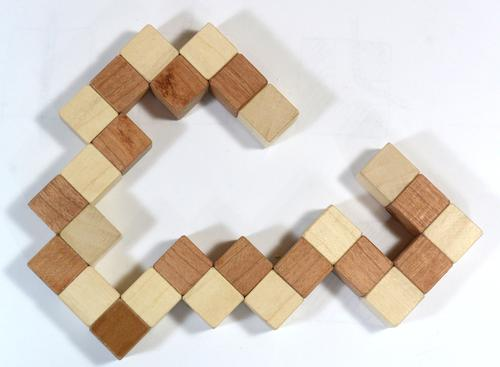
\includegraphics[width=.6\textwidth]{images/snake-cube.jpg}
\end{center}

Oldjuk meg a jól ismert ,,kígyó-kocka'' feladványt!
Az egyes kis szakaszok fixek, de a derékszögű
fordulásoknál egymáson elforgathatóak; a feladat,
hogy kirakjunk belőle egy 3x3-as kockát.

Szokás szerint azzal kezdjük, hogy felvesszük az
adatokat. Ez a készítendő kocka mérete, és a kígyót
alkotó szakaszok hosszai:
\begin{program}
méret(3).
kígyó([3,2,2,3,2,3,2,2,3,3,2,2,2,3,3,3,3]).
\end{program}

A teljes kockán belül minden pozíciót 3
koordinátával tudunk jellemezni:
\begin{program}
pozíció(p(X, Y, Z)) :-
    méret(N), között(1, N, X),
    között(1, N, Y), között(1, N, Z).
\end{program}
Tehát a jelenlegi $3\times3$-as kocka esetében minden
koordináta 1 és 3 között változhat.

A \pr{között} szabály feladatként szerepelt,
így definiálhatjuk:
\begin{program}
között(N, M, N) :- N =< M.
között(N, M, X) :-
    N < M, N1 is N + 1,
    között(N1, M, X).
\end{program}
\index{\pr{között}}
Itt arra érdemes figyelni, hogy \pr{N > M} esetén ez
nem kielégíthető.

Hatféle irányról beszélhetünk, a három tengely
irányában pozitív és negatív irányban. Ezeket
leírhatjuk olyan módon, mint pl. \pr{i(x, -1)} vagy
\pr{i(z, 1)}. Az összes irányt tehát így
fogalmazhatjuk meg:
\begin{program}
irány(i(T,I)) :-
    tartalmaz(T, [x,y,z]),
    tartalmaz(I, [-1,1]).
\end{program}
A \pr{T} itt az egyik tengely, az \pr{I} pedig 1
vagy -1, ami a pozitív ill. negatív irányt jelöli.

Két egymás után következő szakasz mindig merőleges
egymásra, tehát a \emph{tengelyük} nem lehet azonos:
\begin{program}
köv_irány(i(T,_), i(T1,I)) :-
    irány(i(T1,I)), T \= T1.
\end{program}

Hogyan változik egy pozíció, ha ellépünk egy adott
irányban? A \pr{lépés(P1, I, P2)} akkor lesz igaz,
amikor a \pr{P1}-ből \pr{I} irányba ellépve a
\pr{P2}-be jutunk:
\begin{program}
lépés(p(X,Y,Z), i(x,I), p(X1,Y,Z)) :- X1 is X + I.
lépés(p(X,Y,Z), i(y,I), p(X,Y1,Z)) :- Y1 is Y + I.
lépés(p(X,Y,Z), i(z,I), p(X,Y,Z1)) :- Z1 is Z + I.
\end{program}
(Ezért volt jó a pozitív/negatív irányt 1-el és
-1-el jelölni.)

Próbáljuk meg felírni a megoldást! Legyen erre a
szabályunk \pr{megoldás(K, PL, I, X)}; itt \pr{K} a
kígyó hátralevő része, \pr{PL} a már kitöltött
pozíciók listája (az elején a kígyó feje, amit épp
vizsgálunk), az \pr{I} az aktuális irány, és \pr{X}
az irányváltoztatások listája. A reláció akkor
teljesül, ha a \pr{PL} pozíció-lista első elemétől
\pr{I} irányban indulva le tudjuk rakni a \pr{K}
listában levő szakaszokat az \pr{X} listában levő
irányokat követve úgy, hogy mindig a kockán belül
maradunk, és nem megyünk bele a \pr{PL} egyik
elemébe sem. Ekkor a
\begin{query}
?- kígyó(K), pozíció(P), irány(I),
   megoldás(K, [P], I, X).
\end{query}
kérdésre \pr{P} adja a kezdő pozíciót, \pr{I} a
kezdő irányt, és \pr{X} az irányváltoztatásokat.

Ha a kígyónak már csak 1 szakasza van hátra, akkor
csak azt kell megnézni, hogy azt le tudjuk-e tenni:
\begin{program}
megoldás([N], PL, I, [I]) :- ellenőriz(PL, I, N, _).
\end{program}
Az \pr{ellenőriz(PL, I, N, PL1)} akkor lesz igaz, ha
a \pr{PL} elején levő pozícióról az \pr{I} irányban
le tudunk helyezni egy \pr{N} hosszú szakaszt
anélkül, hogy kimennénk a kockából vagy érintenénk
egy \pr{PL}-ben levő pozíciót, és az így bővült
pozíció-lista a \pr{PL1}.

Ezt szavakban elmondani bonyolultabb, mint
programban:
\begin{program}
ellenőriz(PL, _, 1, PL).
ellenőriz([P|M], I, N, PL1) :-
    N > 1, lépés(P, I, P1),
    pozíció(P1), nemtartalmaz(P1, M), N1 is N - 1,
    ellenőriz([P1, P|M], I, N1, PL1).
\end{program}
Ha a szakasz 1 kockából áll, akkor nincs további
teendőnk, és \pr{PL1 = PL}. Egyébként teszünk a
megadott irányban egy lépést, megnézzük, hogy
érvényes pozíció-e, nem szerepel-e az eddigi
pozíciók listájában, és ha ez mind jó, akkor jöhet a
többi lépés -- ehhez a \pr{PL}-et kiegészítjük az új
\pr{P1} pozícióval, és a készítendő szakasz hosszát
csökkentjük 1-el.

Ha a kígyó több szakaszból áll, akkor először
ellépünk az első szakasz hosszával az aktuális
irányban, utána új irányt választunk, és rekurzióval
elvégezzük a maradékot:
\begin{program}
megoldás([N|M], PL, I, [I|X]) :-
    ellenőriz(PL, I, N, PL1), köv_irány(I, I1), 
    megoldás(M, PL1, I1, X).
\end{program}

Ezzel a fent ismertetett módon megkapjuk a
megoldást, de kicsit nehezen olvasható
alakban. Fordítsuk le magyarra az irányokat!
\begin{program}
fordít([], []).
fordít([i(T, I)|M], [F|FM]) :-
    (  T = x, (I = 1, F = jobbra; I = -1, F = balra)
     ; T = y, (I = 1, F = fel;    I = -1, F = le)
     ; T = z, (I = 1, F = előre;  I = -1, F = hátra)
    ), 
    fordít(M, FM).
\end{program}
A \pr{fordít} szabály első argumentuma irányok egy
listája, a második pedig az ennek megfelelő
fordítások listája. Érdemes megfigyelni a
zárójelezés és a logikai vagy jelentésű
pontosvesszők használatát.

Végül akkor tegyük az egész megoldót egy szabályba!
\begin{program}
kígyó_kocka(K, P, FI, FX) :-
    kígyó(K), pozíció(P), irány(I),
    megoldás(K, [P], I, X), fordít([I|X], [FI|FX]).
\end{program}

Ha kipróbáljuk:
\begin{query}
?- kígyó_kocka(K, P, FI, FX).
FI = jobbra,
FX = [jobbra, fel, balra, előre, fel, hátra, jobbra,
      előre, le, balra, fel, hátra, fel, előre, le,
      jobbra, fel],
K = [3, 2, 2, 3, 2, 3, 2, 2, 3, 3, 2, 2, 2, 3, 3, 3,
     3],
P = p(1, 1, 1)
\end{query}
... az eredmény már sokkal könnyebben értelmezhető.

A megoldó elég általános ahhoz, hogy más
változatokra is használható legyen, pl. a ,,mean
green'' feladványra, ha lecseréljük a \pr{kígyó}
definícióját:
\begin{program}
kígyó([3,3,2,3,2,3,2,2,2,3,3,3,2,3,3,3]).
\end{program}
Egy másik variáns a ,,king'' feladvány, amelynél
$4\times4$-es kockát kell építeni:
\begin{program}
méret(4).
kígyó([3,2,3,2,2,4,2,3,2,3,2,3,2,2,2,2,
       2,2,2,2,3,3,2,2,2,2,2,3,4,2,2,2,
       4,2,3,2,2,2,2,2,2,2,2,2,4,2]).
\end{program}
Ennek sokkal több lehetőséget kell megvizsgálnia,
ezért kell neki pár perc.

Megfordíthatjuk a kérdést: hogyan lehet egy
számsorozatot készíteni, ami olyan kígyót határoz
meg, amelyből kocka készíthető? Ehhez a \pr{kígyó}-nak
egy új definíciójára lesz szükségünk:
\begin{program}
kígyó(K) :-
    méret(N), N3 is N^3, N1 is N3 // (N - 1),
    között(N1, N3, H), hossz(K, H),
    kígyó(K, N3).
\end{program}
A teljes kígyó hossza a méret köbe (\pr{N3}). A
kígyót alkotó szakaszok száma (a kígyónak, mint
szakasz-listának a \emph{hossza}, \pr{H}) tehát
\pr{N3/(N-1)} és \pr{N3} között lesz, hiszen minden
szakasz legfeljebb \pr{N-1} új pozíciót fedhet
le. Az egyes szakaszokat ezután a \pr{kígyó/2}
segítségével készítjük el:
\begin{program}
kígyó([], 1).
kígyó([Sz|K], M) :-
    M > 1, méret(N), között(2, N, Sz),
    M1 is M - Sz + 1, kígyó(K, M1).
\end{program}
Ha még \pr{M} hosszú kígyót kell csinálni, akkor
választunk egy számot 2 és \pr{N} között (egy
szakasz hossza csak ilyen lehet), ez lesz a mostani
szakaszunk hossza, és a maradék szakaszokkal pedig
egy ennyivel rövdebb kígyót csinálunk (pontosabban
eggyel hosszabbat, mert egy szakasz utolsó eleme
egyben a következő első eleme). Amikor már csak 1
hosszú kígyót kell csinálni, készen vagyunk.

Ezzel a definícióval azt kapjuk, hogy
\begin{query}
?- kígyó_kocka(K, P, FI, FX).
K = [2, 3, 3, 2, 3, 3, 3, 3, 3, 3, 3, 2, 3, 2, 3],
P = p(1, 2, 2),
FI = le,
FX = [le, jobbra, fel, hátra, le, balra, fel, előre,
      le, jobbra, fel, balra, hátra, le, előre] 
\end{query}
(Ez jó sokáig tart.) Mivel a szakaszok számával
alulról felfele próbálkozunk, az első megoldás a
legkevesebb szakaszból álló kígyó (15 db), amit
$3\times3$-as kockába lehet rendezni. Ha a fenti
definícióban a \pr{között(N1, N3, H)} helyett \pr{H
  = 15}-öt írunk (tehát ha lerögzítjük a szegmensek
számát), akkor gyorsan lefut.

A futási idő mindig egy kompromisszum: (aránylag)
keveset kellett gondolkodnunk ahhoz, hogy megírjuk
ezt a programot. Hatékonyabb programot gyakran
nehezebb írni, viszont néha elég a lassabb is,
pl.~olyan feladatoknál, mint a kígyó-generálás,
amikor a lényeg csak az, hogy találjunk egy
megoldást (még ha akár napokig is kell a gépnek
számolnia). Azért persze törekedjünk a
hatékonyságra!

\subsection*{A teljes program}

Mivel ez már egy elég összetett program volt, itt
van egyben az egész:

\begin{program}
tartalmaz(X, [X|_]).
tartalmaz(X, [_|M]) :- tartalmaz(X, M).

nemtartalmaz(_, []).
nemtartalmaz(X, [Y|M]) :- X \= Y, nemtartalmaz(X, M).

hossz([], 0).
hossz([_|M], N) :- hossz(M, N1), N is 1 + N1.

között(N, M, N) :- N =< M.
között(N, M, X) :-
    N < M, N1 is N + 1,
    között(N1, M, X).

% Standard
méret(3).
kígyó([3,2,2,3,2,3,2,2,3,3,2,2,2,3,3,3,3]).

% Mean green
% méret(3).
% kígyó([3,3,2,3,2,3,2,2,2,3,3,3,2,3,3,3]).

% King
% méret(4).
% kígyó([3,2,3,2,2,4,2,3,2,3,2,3,2,2,2,2,
%        2,2,2,2,3,3,2,2,2,2,2,3,4,2,2,2,
%        4,2,3,2,2,2,2,2,2,2,2,2,4,2]).

% Generáló
% méret(3).
% kígyó(K) :-
%     méret(N), N3 is N^3, N1 is N3 // (N - 1),
%     között(N1, N3, H), hossz(K, H),
%     kígyó(K, N3).
% kígyó([], 1).
% kígyó([Sz|K], M) :-
%     M > 1, méret(N), között(2, N, Sz),
%     M1 is M - Sz + 1, kígyó(K, M1).

pozíció(p(X, Y, Z)) :-
    méret(N), között(1, N, X),
    között(1, N, Y), között(1, N, Z).

irány(i(T,I)) :-
    tartalmaz(T, [x,y,z]),
    tartalmaz(I, [-1,1]).

köv_irány(i(T,_), i(T1,I)) :-
    irány(i(T1,I)), T \= T1.

lépés(p(X,Y,Z), i(x,I), p(X1,Y,Z)) :- X1 is X + I.
lépés(p(X,Y,Z), i(y,I), p(X,Y1,Z)) :- Y1 is Y + I.
lépés(p(X,Y,Z), i(z,I), p(X,Y,Z1)) :- Z1 is Z + I.

ellenőriz(PL, _, 1, PL).
ellenőriz([P|M], I, N, PL1) :-
    N > 1, lépés(P, I, P1),
    pozíció(P1), nemtartalmaz(P1, M), N1 is N - 1,
    ellenőriz([P1, P|M], I, N1, PL1).

megoldás([N], PL, I, [I]) :- ellenőriz(PL, I, N, _).
megoldás([N|M], PL, I, [I|X]) :-
    ellenőriz(PL, I, N, PL1), köv_irány(I, I1), 
    megoldás(M, PL1, I1, X).

fordít([], []).
fordít([i(T, I)|M], [F|FM]) :-
    (  T = x, (I = 1, F = jobbra; I = -1, F = balra)
     ; T = y, (I = 1, F = fel;    I = -1, F = le)
     ; T = z, (I = 1, F = előre;  I = -1, F = hátra)
    ), 
    fordít(M, FM).

kígyó_kocka(K, P, FI, FX) :-
    kígyó(K), pozíció(P), irány(I),
    megoldás(K, [P], I, X), fordít([I|X], [FI|FX]).
\end{program}
